\chapter{Workload-Aware Data Placement}
\label{chapter:dp}

A CAT optimizer determines the best architectural choices.
For example, users can scale out or shrink in a cluster size to meet workload changes.
In this chapter, we focus on optimizing performance after a software system
is reconfigured.

% Claims
% 1. Uniform elasticity is suboptimal in many cases
% 2. Workload-aware data placement increases the system performance
%    - coarse-grained: 15% for powerlaw workload distribution (common workload)
% 3. Placement strategy (to show the tradeoff)
%    - increasing color span (rainbow) → better balancing workload
%    - minimizing color span (monochromatic) → largely exploting caching locality
% 4. Hybrid placement strategy shows both advantages

\section{Introduction}
\label{sec:introduction}

In large-scale, distributed systems the dataset, which is too large
for a single node, is partitioned among the nodes.
Incoming workload (\emph{i.e.,} requests) is routed among nodes by a
load balancer.
For extreme horizontal scaling to be effective, it is necessary for
nearly all requests to be routed to a node containing the needed data
locally, which avoids unnecessary node-to-node interactions.
Consequently, data replication and data placement are components of load
balancing and have a substantial impact on system performance.
In the literature, for example,
AUTOPLACER \cite{Rodrigues2013} and MET \cite{Cruz2013}
optimize data placement to fit workload characteristics in NoSQL databases.
Replicating hotter data in storage is a common approach
to balance load \cite{Lim2010}.
In relational databases, sharding is used to distribute load
by partitioning tables to achieve effective horizontal scaling
\cite{Chang2008, george2011hbase, Lakshman2010, Adya2016, Curino2010}.


Cloud computing has changed how computing resources are used.
Before cloud computing, infrastructure is purchased and used for many
years before it is upgraded or replaced.
However, with Infrastructure as a Service (IaaS) equipment is rented
for a short time, including as short as one execution of an
application.
This shift from buying to renting greatly increases the flexibility of
infrastructure available for a given application.
Therefore, rather than tune an application to run well on a specific
machine, a cloud user instead can tune the
infrastructure to accommodate each application on each
dataset.
When an infrastructure is resized in response to changes in workloads,
it is necessary to replicate and place data partitions among nodes.
It is still unclear what are the better strategies
for this decision---prior work on data placement
does not totally address these issues~\cite{Rodrigues2013, Cruz2013, Lim2010}.


Efficient deployment of distributed systems with an
irregular workload requires both cluster sizing and
data placement.
N\"aive uniform data replication (where all data partitions have the
same number of replicas) is effective only when the workload is also
uniform---requests are equally distributed among all partitions.
\emph{Workload-aware} data placement replicates and places
partitions to match the distribution of requests in the anticipated
workload.

\begin{figure}[!htbp]
    \centering
    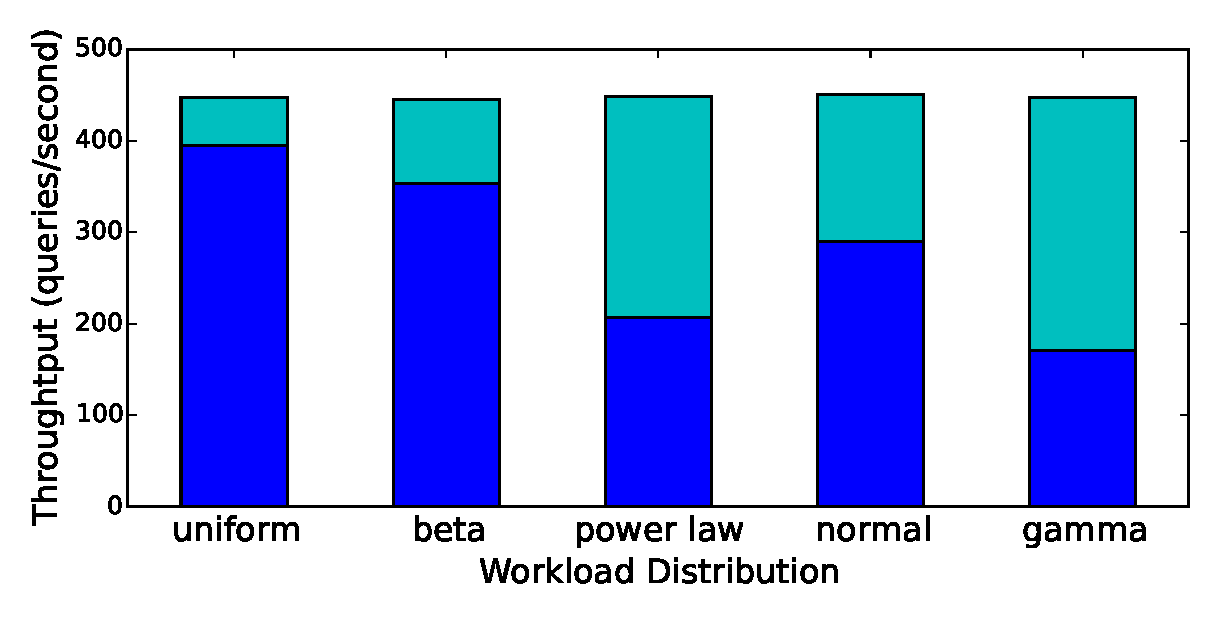
\includegraphics[width=0.8\linewidth]{figures/E34_uniform_suboptimal_tp_stacked_scdm2017.eps}
    \caption{Uniform data placement is suboptimal.
             The lower bar is the measured throughput of uniform placement while
             the upper bar is the performance loss to the idealistic placement.
(Data is a subset of data shown in
\mytable{\ref{tab:throughput_comparison_local}} on Section~\ref{sec:evaluation}.)}
    \label{fig:uniform_suboptimal}
\end{figure}

\myfigure{\ref{fig:uniform_suboptimal}} illustrates the cost of
uniform data replication on non-uniform workloads.
The results for five different workloads are presented on the $x$-axis;
the skew (degree of imbalance) in the workload increases from
left to right.
The \emph{complete} placement solution, where each node has all data,
is an idealistic upper bound on the potential gains of
matching data replication and workload.
% Uniform placement is within 10\% of ideal when the workload is
% uniform.
Because any node can process a request, new requests are sent to the
least loaded node and the performance of \emph{complete} is flat across all
workloads.
In this example, the cluster has twice the minimum capacity, so uniform
replication has two copies of each partition.
Therefore, a request must be sent to
one of the two nodes that hold the data associated
with the request.
Throughput decreases as the
workload skew increases because some nodes are over loaded and
others are under utilized.
While uniform placement achieves 88\% of ideal on uniform workload, it
is only 38\% of ideal on the highly-skewed gamma workload.
This example illustrates the need to properly \emph{replicate} and
\emph{place} data on the nodes of a cluster.


This chapter explores the three dimensions that affect data placement.
The first dimension is \emph{granularity} of data partitions.
Fine-grain (more than one partition per node) placement has costs
(overhead) and benefits (flexibility).
The second dimension is how many \emph{replicas} of each partition.
We let the anticipated demand per partition (\emph{i.e.}, the
\emph{workload}) 
determine the replication factor for each data partition.
The hotter the data, the greater the replication.
The number of data partitions influences how closely the replication
matches the workload.
However,
a coarse-grain partition (one per node) is unlikely to match the
workload.
Last, fine-grain partitioning introduces the
\emph{placement} dimension because there are several ways to distribute
the partitions among the nodes.

We present results from a simulation program that
examines these three dimensions.
We find that coarse-grain placement does not provide sufficient
flexibility to balance non-uniform loads.
A surprisingly small amount of additional partition granularity
is sufficient to load balance and obtain most benefits.
The work presents and evaluates the tradeoff between several
fine-grain placement strategies that either
increase robustness to tolerate workload deviation or
reduce storage footprint.

To further examine these conclusions, our empirical study
on an HPCC cluster\footnote{HPCC Systems is an open source
  \emph{data-analytics computer}---a highly scalable, distributed
  framework for processing and analyzing
  large datasets---supported by LexisNexis Risk Solutions at
  \url{https://hpccsystems.com/}.
}
shows that proper data replication and placement
affect system performance greatly.
The coarse-grain scheme improves system throughput by
$25\%$ and $85\%$ for the normal and power law distribution,
respectively.
A fine-grain placement strategy 
improves query throughput by $52\%$ and $105\%$.
On the most highly-skewed case, the improvement is $166\%$ increase over the
n\"aive solution.

Because data placement relies on a prediction of the upcoming
workload, which will invariably be wrong to some degree.
This chapter, therefore, considers the \emph{robustness}, which
is a measure to describe how sensitive a data placement scheme is to
slightly mis-predicted workloads, of several placement strategies.
Results show that maximizing the number of unique partitions per node
increases the robustness of a placement.
\section{Modeling Data Replication and Placement}
\label{sec:model}

Our work concerns systems in which the dataset
must be partitioned among the nodes because the dataset
is too large to be completely
replicated on each node.
We replicate subsets of the whole dataset in order to increase
throughput and decrease latency.
While replication for availability is critically important, it is not a
subject of this research. 

Distributed, large-scale systems such as
Apache Hadoop, Spark, Cassandra, and Ceph
largely exploit data locality while reducing node-to-node
communication for achieving high horizontal
scaling~\cite{DeanJ2004_MapReduce,zaharia2010spark,Lakshman2010,SageWeil2006Ceph}. 
Data partitions are replicated as the system scales out.
An inefficient data placement scheme is unable to achieve the
optimal system performance and service-level objective (SLO)
violations may occur~\cite{Rodrigues2013,Cruz2013,Trushkowsky2011,Majors2010}.

The goal of this work is to place data partitions onto nodes such
that the performance is maximized for the upcoming workload.
There is a large body of work supporting workload
prediction~\cite{Gmach2007,box2015time,Akdere2012}.
This work assumes that a reliable (though not
necessarily perfect) prediction is provided by some other work.
Instead of solely relying on accurate workload prediction,
systems can dynamically adjust replication factors
and data locations for handling workload changes
~\cite{Lim2010, Trushkowsky2011, Cruz2013}.
This work focuses on determining the optimal
partition granularity, replication factors, and placement strategy.
Our work is complementary to a dynamic approach.

The following model characterizes the 
\emph{data replication and placement problem} in large-scale,
distributed systems. 
Let $M>1$ be the minimum cluster size that is sufficient to hold all
data.
The storage capacity is strictly limited by the amount of data it
physically can store locally.
In many real-world applications, $M$ is in the hundreds of nodes.
However, for this model it is only necessary that $M$ not be equal to
one, which does not require data partitioning.

Let $N$ ($N \ge M$) be the number of nodes in a cluster.
When the workload changes, the cluster expands ($N$ increases)
to meet increased demand and minimize QoS violations, or it contracts
($N$ decreases) to reduce resources and cost. 
But the cluster cannot contract smaller than the $M$ nodes needed to
hold the data.

The data is partitioned into $k \ge 1$ equal-sized data partitions on each node.
Thus, the dataset has $P = Mk$ unique partitions.
Because the cluster has $N$ nodes, there are $S = Nk$ \emph{slots} for
data partitions.
We define the \emph{replication factor}, $R$, as $R=N/M$.
When $R>1$, then $N>M$ and $S > P$ and some partitions will
be replicated among
the ``extra'' slots.
\emph{Coarse-grain} data placement occurs when there is only one
partition per node, $k=1$.
\emph{Fine-grain} data placement, $k>1$, which has more total
data partitions and partition slots, supports more distinct placements
than coarse-grain providing a better opportunity to match the
workload, and increases performance.

\medskip
\begin{tabular}[h]{lll}
  \multicolumn{3}{l}{\textbf{Model parameters}}\\
  ~~~~&\emph{Minimum number of nodes:} & $M>1$\\
  &\emph{Per node granularity:} & $k\ge 1$ \\
  &\emph{Replication factor:} & $R\ge 1$ \\
  \multicolumn{3}{l}{\textbf{Derived terms}}\\
  &\emph{Instantiated nodes:} & $N=RM$\\
  &\emph{Unique data partitions:} & $P = Mk$\\
  &\emph{Slots:} & $S = Nk = RMk$\\
\end{tabular}
\medskip

We present a motivating example below.
The base cluster has four nodes, $M=4$.
The current demand is twice the current capacity.
\myfigure{\ref{fig:dp_before_coarse}}
shows the load per partition on four nodes.
The load is unevenly distributed among the partitions.
In particular, in terms of node capacity the load on the four partitions in
\myfigure{\ref{fig:dp_before_coarse}} is 3.5, 2, 1.5, and 1 (which
conveniently totals 8).
\myfigure{\ref{fig:dp_before_fine}}, shows the same
aggregate demand as it is distributed among 16 partitions, four per
node: $k=4$.
Fine-grain replication gives rise to a \emph{placement} decision.
Redistributing loads helps reduce load imbalance among nodes
by placing highly requested partitions onto least loaded nodes.
In \myfigure{\ref{fig:dp_before_fine_placement}} the load is nearly
balanced: two nodes have a load of 2.125 and two have 1.875.
However, this alone does not help solve the overloading issue
because the workload demand is twice the system capacity.

Suppose the cluster doubles in size to eight nodes exactly meeting
anticipated demand: $R=2$ and $N=8$.
Uniform replication onto eight nodes creates two replicas of each
partition as shown in \myfigure{\ref{fig:dp_uniform}}.
The red box above the two left-most nodes shows the excess demand on those
nodes as 3.5 units of node capacity are serviced by two nodes.
The white regions in the four right-most nodes show the
underutilization because the demand is less than the capacity.

A coarse-grain, non-uniform solution is clearly better
than uniform because \emph{hotter} partitions can be
replicated more than \emph{colder} ones.
For example, in \myfigure{\ref{fig:dp_coarse}} the 3.5 units of P1 are
distributed over three nodes.
Unsurprisingly, a fine-grain solution can better match the demand to
the capacity.
\myfigure{\ref{fig:dp_fine_monochromatic}} shows that demand is perfectly matched to
capacity in this idealized example.


\myfigure{\ref{fig:dp_fine_rainbow}} shows a second placement that also
perfectly balances load but has four unique partitions on each
node.
The nodes in \myfigure{\ref{fig:dp_fine_monochromatic}} have either
one or two unique partitions.
Fewer unique partitions per node reduces the footprint of both primary
(memory) and secondary (disk) storage.
On the other hand,
more unique partitions per node increases the number of nodes that can
respond to a given request, which may better share the load among nodes.

This simple example was constructed to clearly show
the benefits of non-uniform, fine-grain data placement.
Unless the demand is uniformly distributed among the partition (an
extremely unlikely occurrence as explained in
Section~\ref{sec:workloads}) then a n\"aive uniform placement leads to
over- and underutilization.


\begin{figure}[!htbp]
\begin{subfigure}[b]{0.75\textwidth}
    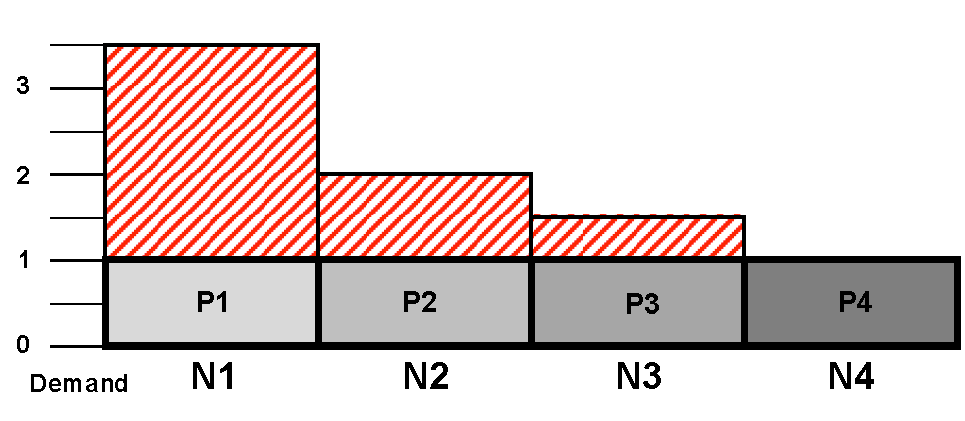
\includegraphics[width=\linewidth]{figures/dp_final_before_coarse.pdf}
    \caption{Coarse-Grain ($M=4,R=1,k=1$)}
    \label{fig:dp_before_coarse}
\end{subfigure}
\begin{subfigure}[b]{0.75\textwidth}
    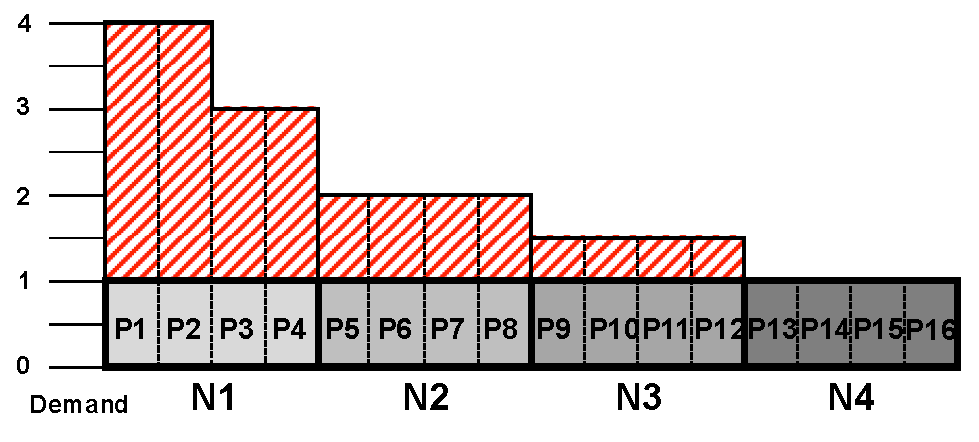
\includegraphics[width=\linewidth]{figures/dp_final_before_fine.pdf}
    \caption{Fine-Grain ($M=4,R=1,k=4$)}
    \label{fig:dp_before_fine}
\end{subfigure}
\begin{subfigure}[b]{0.75\textwidth}
    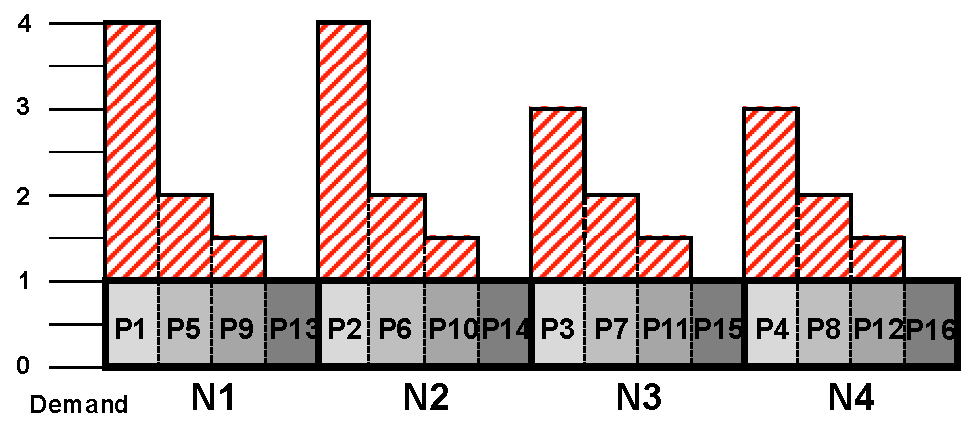
\includegraphics[width=\linewidth]{figures/dp_final_before_fine_R1.pdf}
    \caption{Fine-Grain alternative placement}
    \label{fig:dp_before_fine_placement}
\end{subfigure}
\centering
\caption{The workload demand exceeds the system capacity.}
\label{fig:dp_before}
\end{figure}


\begin{figure}[!htbp]
\begin{subfigure}[b]{0.9\textwidth}
    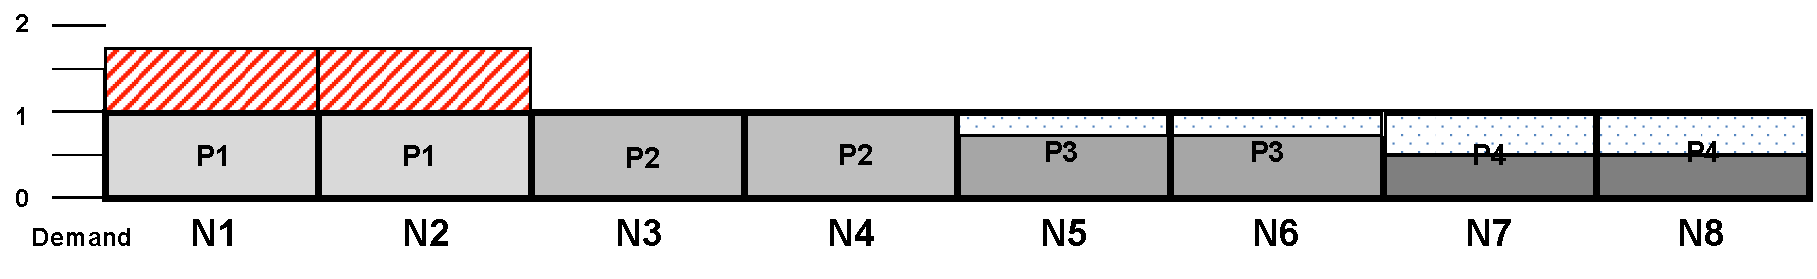
\includegraphics[width=\linewidth]{figures/dp_final_uniform.pdf}
    \caption{Uniform data placement ($M=4,R=2,k=1$)}
    \label{fig:dp_uniform}
\end{subfigure}
\hfill
\begin{subfigure}[b]{0.9\textwidth}
    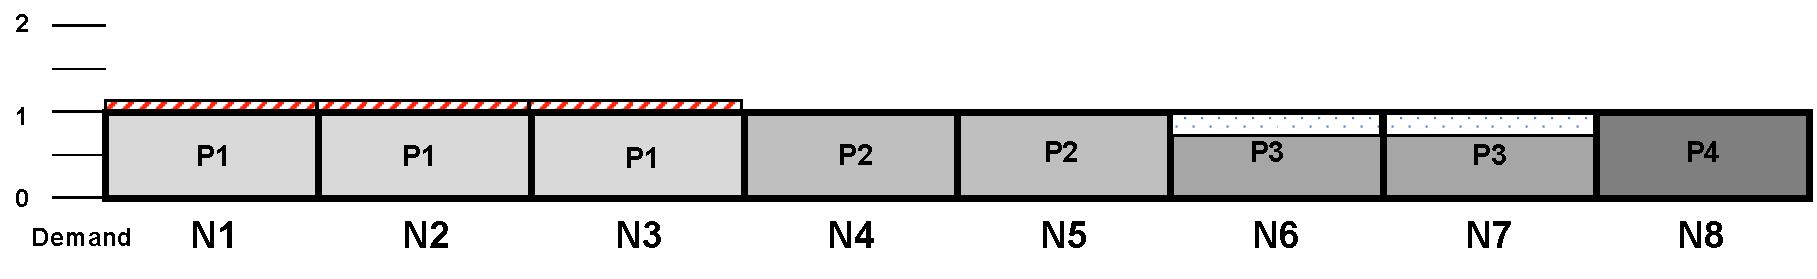
\includegraphics[width=\linewidth]{figures/dp_final_coarse.pdf}
    \caption{Coarse-grain data placement ($M=4,R=2,k=1$)}
    \label{fig:dp_coarse}
\end{subfigure}
\hfill
\begin{subfigure}[b]{0.9\textwidth}
    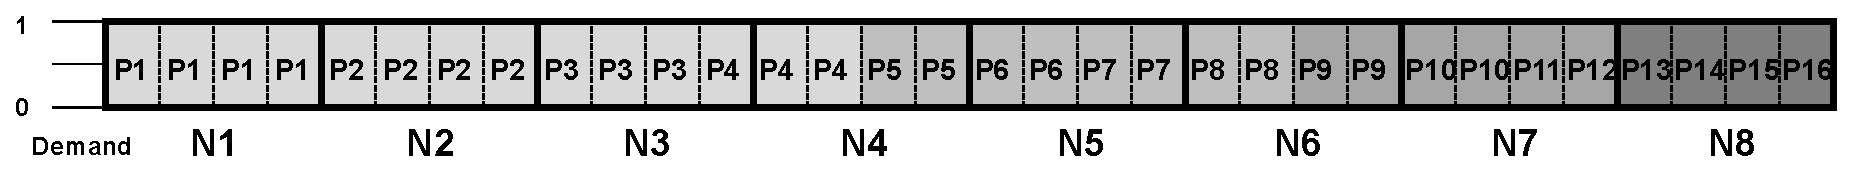
\includegraphics[width=\linewidth]{figures/dp_final_fine_monochromatic.pdf}
    \caption{Fine-grain \emph{compact} data placement ($M=4,R=2,k=4$)}
    \label{fig:dp_fine_monochromatic}
\end{subfigure}
\hfill
\begin{subfigure}[b]{0.9\textwidth}
    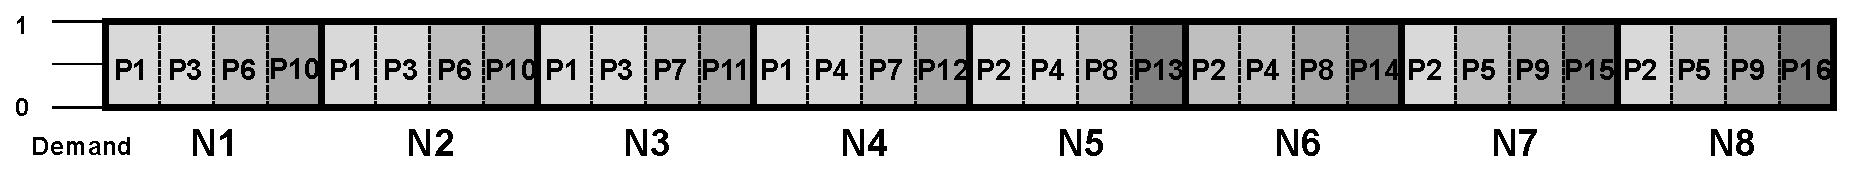
\includegraphics[width=\linewidth]{figures/dp_final_fine_rainbow.pdf}
    \caption{Fine-grain \emph{balanced} data placement ($M=4,R=2,k=4$)}
    \label{fig:dp_fine_rainbow}
\end{subfigure}
\centering
\caption{Different data placement schemes.}
\label{fig:dp_schemes}
\end{figure}

\section{Workloads}
\label{sec:approach}

This section presents the data placement problem.
First, it characterizes the workloads used in the work.
Next, it expounds on the three dimensions of the problem:
(1) granularity, (2) replication, and (3) placement.
Last, it explains and analyzes three data placement methods,
comparing
performance in terms of load imbalance, storage footprint, and robustness.

\subsection{Workload Characteristics}
\label{sec:workloads}

A workload can be described with several critical characteristics,
such as arrival rate and autocorrelation.
Because this work considers data replication and placement, 
the workload characteristic that matters most is access frequency of the
individual elements of the
dataset, such as, the pages of a web server or the keys in an index.
Other characteristics are not factored into
this work because they do not have a direct impact on data replication
or placement.

A uniform workload is atypical and likely artificial,
which is unsurprising because
non-uniform workloads are common in many natural settings
~\cite{Pavlo2012}.
For example, the normal (Gaussian) distribution can be observed
in class score distribution,
while the log-normal distribution is useful to describe
the response file size in web servers~\cite{Barford1998}.
In addition, the power law probability distribution is widely applicable to
web hits, word frequency, personal income, \emph{etc}.\ and tends to
be highly skewed towards a small subset of the full
dataset~\cite{Newman2005}.
That is, a small number of partitions accounts the vast majority of key access
and most of the partitions are touched infrequently. 
Several studies show that frequency of access to different pages or
keys often follows a Zipf or power law distribution.
This has been shown in web servers~\cite{dilley1998web,panteleenko2003web},
video streaming~\cite{sripanidkulchai2004analysis}, 
and Wikipedia traffic~\cite{urdaneta2009wikipedia} to name a few.

In this work, we consider the
\emph{normal} and the \emph{power law} distribution for their
wide appearance in many workloads.
We also consider the \emph{uniform} distribution for a n\"aive baseline,
\emph{beta}, which is less skewed than
\emph{normal} and \emph{power law}, and
\emph{gamma}, which generates the highest skewed workload and
has been used in modeling workloads in storage systems~\cite{Wilkes2001}.


\mytable{\ref{tab:load-imbalance}} shows
the five workload distributions used in the work.
This table presents the distribution of the
requests on each of four partitions ($M=4$, $k=1$).
There are 30,000 unique requests among the 1024 keys,
and the average is 7,500 requests per partition.
The requests-per-node values are ordered in decreasing magnitude.
As expected there are approximately the same number of requests for
each partition in the uniform distribution.
The \emph{max:mean} column shows the ratio of the maximum number of requests
to the average.
Because the total running time is largely dependent on the slowest or
most heavily loaded node, the max-mean ratio foretells the performance
penalty for each workload on a uniform distribution.
The ratio for uniform is 1.01, meaning the maximum is 1\% greater
than the average.
But the highly-skewed gamma distribution has one partition that receives
no requests and one has more than three times the average.
It is clear from \mytable{\ref{tab:load-imbalance}} that in
non-uniform workloads
the maximally loaded partition demands
more resources than the other partitions.
The final column presents access imbalance using the 
\emph{skew} metric~\cite{Pavlo2012}. 

This work evaluates the problem using synthetic workloads.
An alternative is to evaluate using real-world traces.
But such traces are in short supply.
Moreover, a trace represents a very specific situation that may not be
representative of a general class.
Additionally, a trace has many characteristics that are hard to
control.
Using synthetic workloads enables us to evaluate more distributions and
confine the observed effects to the change in distribution.


\begin{figure}[!htbp]
\begin{subfigure}[b]{0.45\textwidth}
    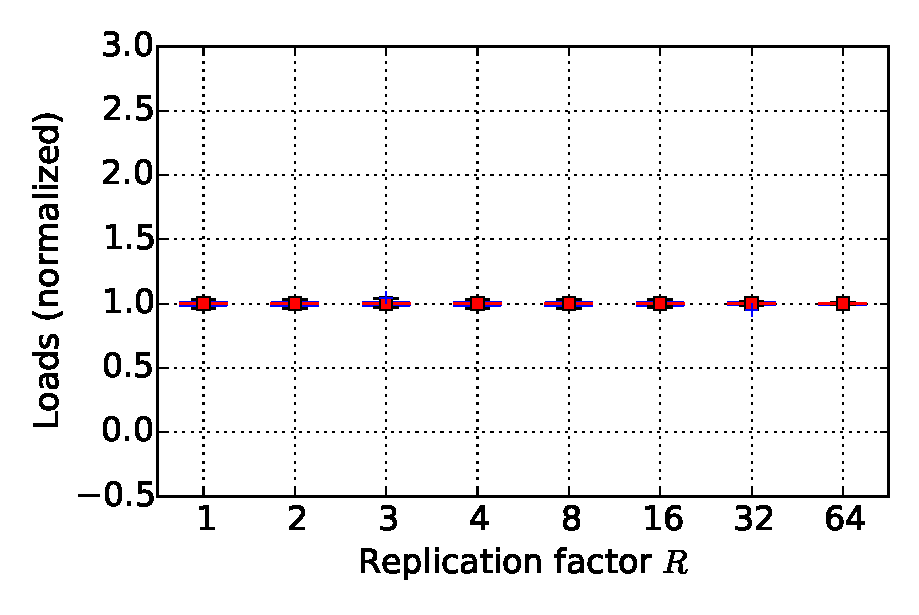
\includegraphics[width=\linewidth]{figures/E45_simulation_imbalance_coarse_std_uniform.eps}
    \caption{uniform}
\end{subfigure}
\begin{subfigure}[b]{0.45\textwidth}
    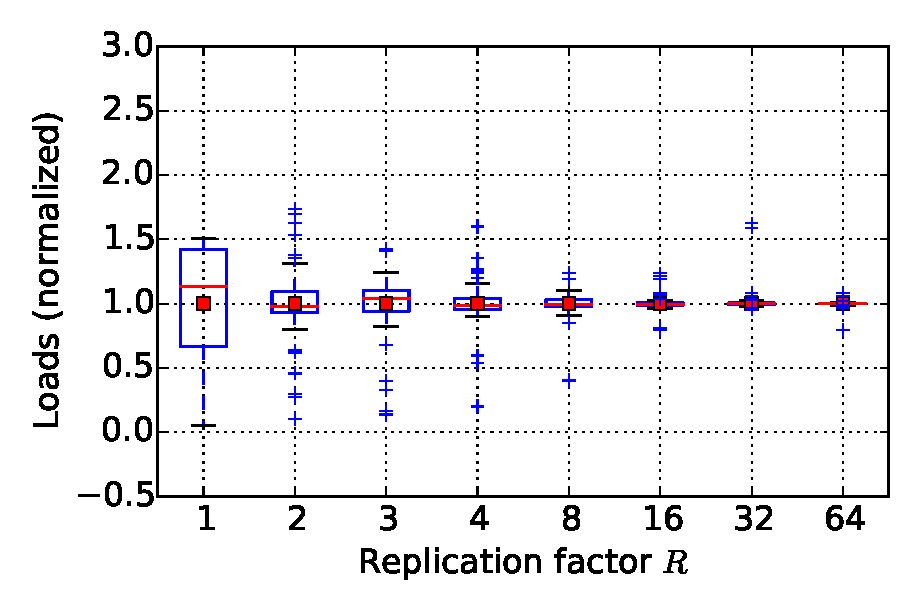
\includegraphics[width=\linewidth]{figures/E45_simulation_imbalance_coarse_std_beta.eps}
    \caption{beta}
\end{subfigure}
\begin{subfigure}[b]{0.45\textwidth}
    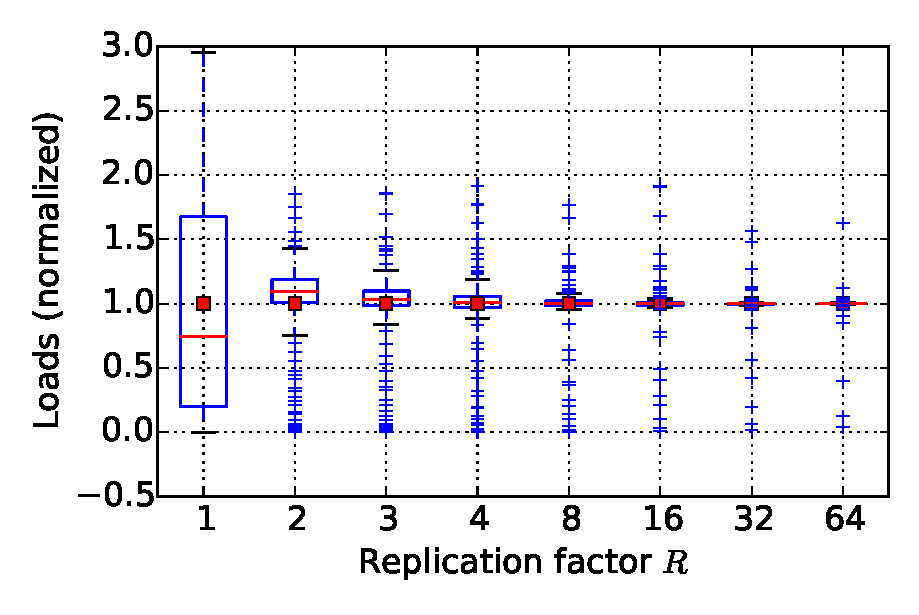
\includegraphics[width=\linewidth]{figures/E45_simulation_imbalance_coarse_std_powerlaw.eps}
    \caption{power law}
\end{subfigure}
\begin{subfigure}[b]{0.45\textwidth}
    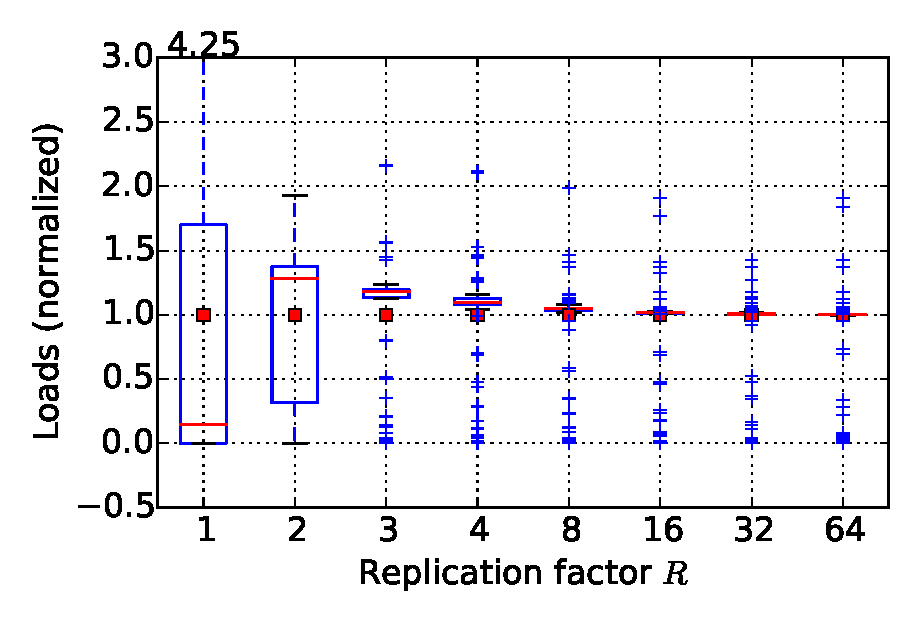
\includegraphics[width=\linewidth]{figures/E45_simulation_imbalance_coarse_std_normal.eps}
    \caption{normal}
\end{subfigure}
\begin{subfigure}[b]{0.45\textwidth}
    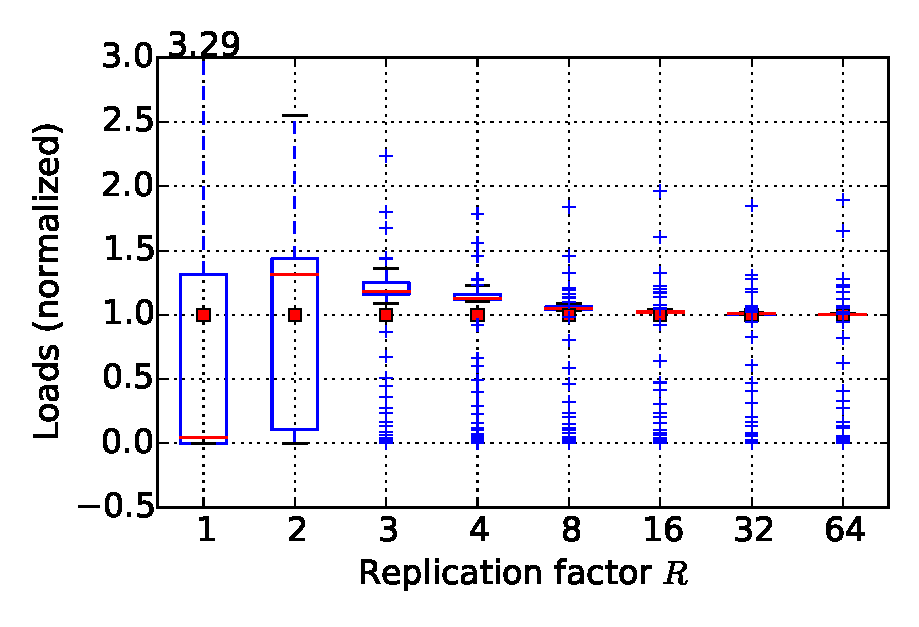
\includegraphics[width=\linewidth]{figures/E45_simulation_imbalance_coarse_std_gamma.eps}
    \caption{gamma}
\end{subfigure}
\centering
\caption{The load distribution among nodes under the coarse-grain data placement ($M=64, k=1$).}
\label{fig:simulation_imbalance_coarse}
\end{figure}


\begin{figure}[!htbp]
\begin{subfigure}[b]{0.45\textwidth}
    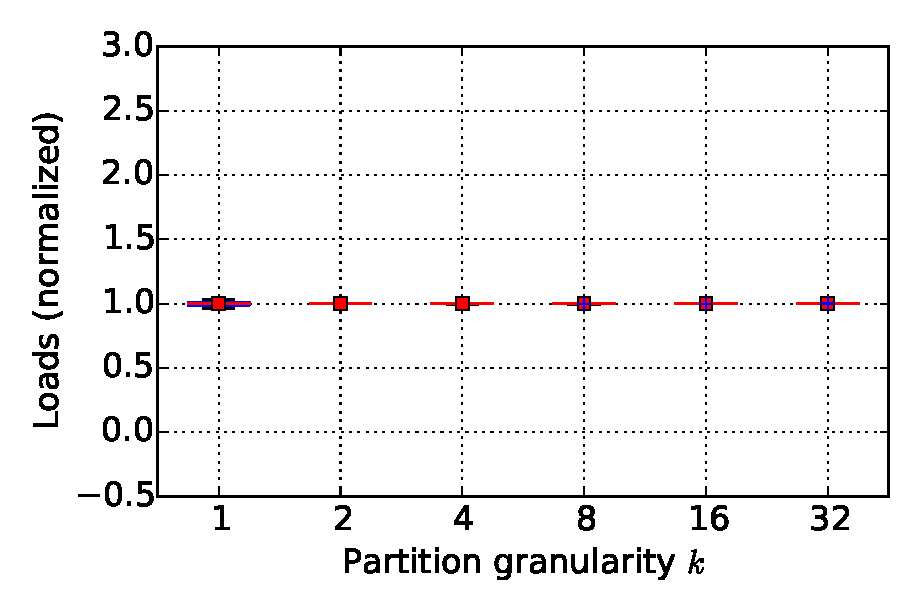
\includegraphics[width=\linewidth]{figures/E45_simulation_imbalance_fine_std_uniform.eps}
    \caption{uniform}
\end{subfigure}
\begin{subfigure}[b]{0.45\textwidth}
    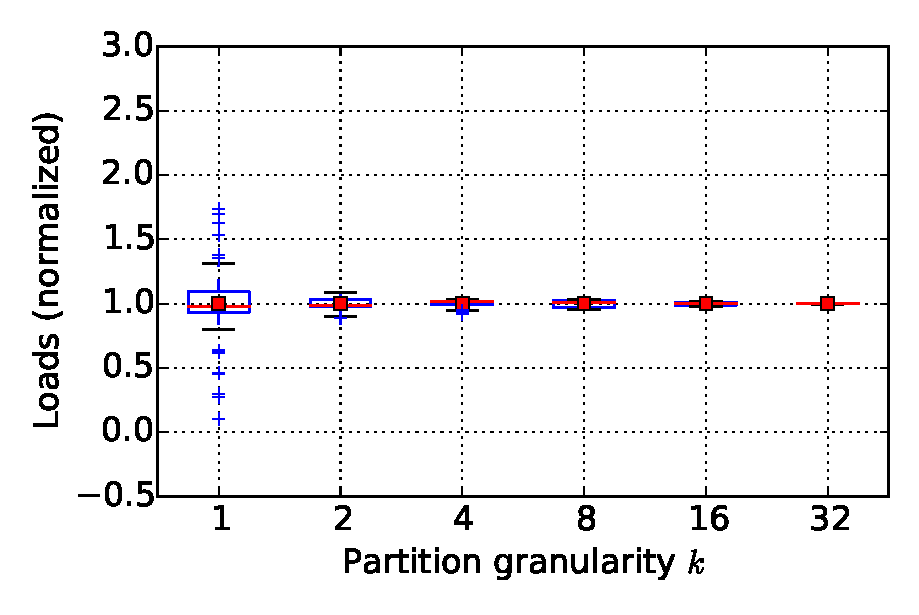
\includegraphics[width=\linewidth]{figures/E45_simulation_imbalance_fine_std_beta.eps}
    \caption{beta}
\end{subfigure}
\begin{subfigure}[b]{0.45\textwidth}
    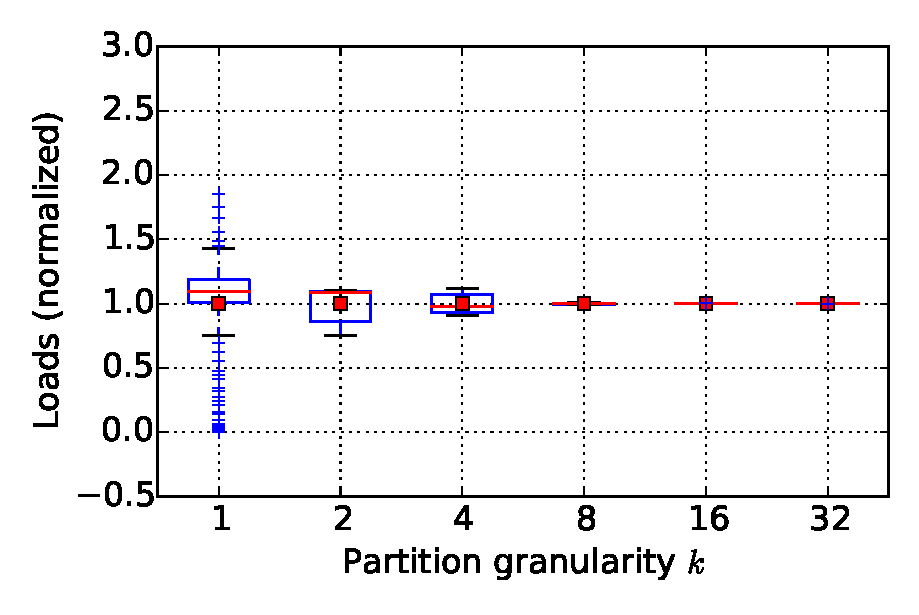
\includegraphics[width=\linewidth]{figures/E45_simulation_imbalance_fine_std_powerlaw.eps}
    \caption{power law}
\end{subfigure}
\begin{subfigure}[b]{0.45\textwidth}
    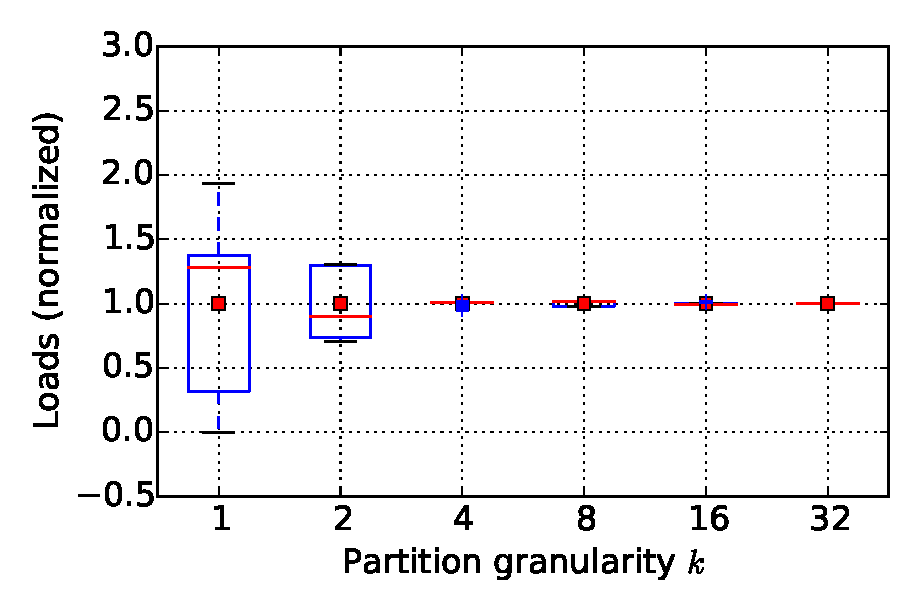
\includegraphics[width=\linewidth]{figures/E45_simulation_imbalance_fine_std_normal.eps}
    \caption{normal}
\end{subfigure}
\begin{subfigure}[b]{0.45\textwidth}
    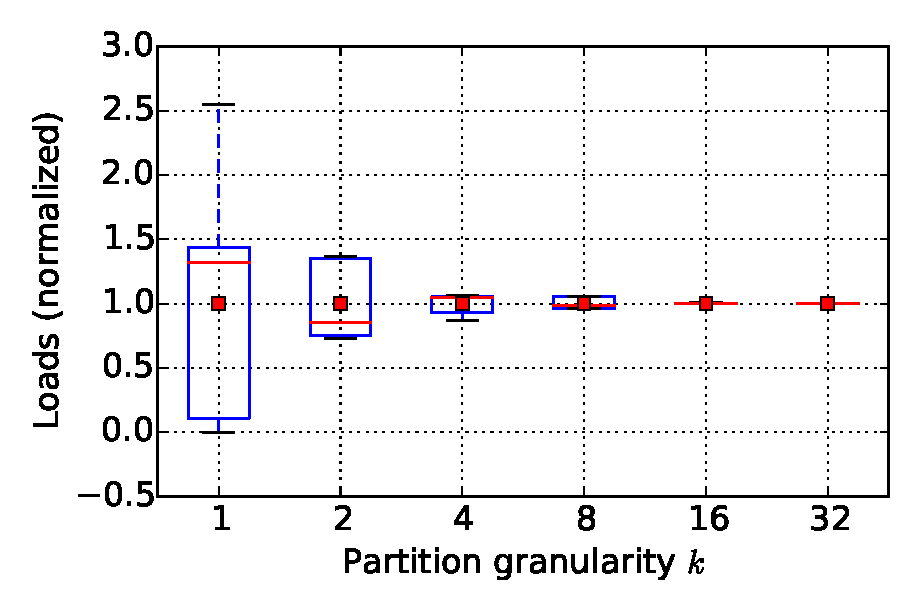
\includegraphics[width=\linewidth]{figures/E45_simulation_imbalance_fine_std_gamma.eps}
    \caption{gamma}
\end{subfigure}
\centering
\caption{The load distribution among nodes under the fine-grain data placement with various $k$ ($M=64, R=2$).}
\label{fig:simulation_imbalance_fine}
\end{figure}


\begin{table}[!htbp]
  \centering
  \caption{Load-imbalance of workloads.}
  \resizebox{\columnwidth}{!}{%
  \begin{tabular}[h]{lrrrrcc}
    \toprule
Distribution & 	\multicolumn{4}{l}{Requests for individual partitions}
    & max:mean & skew\\
\midrule
Uniform & \textbf{7,565} & 7,548 & 7,449 & 7,438 & 1.01 & 0.15\\
Beta & \textbf{10,313} & 10,288 & 4,715 & 4,684 & 1.38 & 0.39\\
Power law & \textbf{17,344} & 8,795 & 3,361 & 500 & 2.31 & 0.60 \\
Normal & \textbf{14,882} & 14,827 & 149 & 142 & 1.98 & 0.74\\
Gamma & \textbf{23,542} & 6,329 & 129 & 0 & 3.14 & 0.77\\
\bottomrule
  \end{tabular}
  }
  \label{tab:load-imbalance}
\end{table}


%%%%%%%%%%%%%%%%%%%%%%%%%%%%%%%%%%%%%%%%
% Approaches
%%%%%%%%%%%%%%%%%%%%%%%%%%%%%%%%%%%%%%%%

\subsection{Data Placement Steps}
\label{sec:dp_methods}

A data placement method requires determining
partition granularity, replication factors, and placement schemes.
Partition granularity represents the smallest unit
for replicating data and calculating loads.
The coarsest granularity is one partition per node ($k=1$), and
the finest is one partition per key.
A small $k$ decreases the likelihood of balancing a non-uniform workload.
However, a large $k$ increases management overhead.

Once the partition granularity $k$ is determined,
the next step
in deriving a solution is determining the number of
replicas for each partition based on the expected workload.
For example, suppose there are four partitions ($P=4$) with a
replication factor of four ($R=4$), then
there are sixteen slots for these partitions ($S=16$) in a
coarse-grain solution.
Given a uniform expected workload the replication factor vector would be 
[4, 4, 4, 4], that is there are four copies of each of the four
partitions. 
For a workload with a normal distribution the replication factor
vector might be [2, 6, 6, 2] and for 
power law it might be [1, 2, 4, 9].
In general, there is no perfect match between the vector and the
anticipated workload.

Assuming that the predicted load on each partition is $\lambda_i$ and the total
load is $\Lambda = \sum_{i=1,P}\lambda_i$.
The replication problem is to determine the \emph{replication vector},
$\vec{R}, R_i \in \mathcal{I}$, such that
$R_i \ge 1~\forall i$  and
$S = \sum_{i=1,P}R_i$.
In words, the replication vector contains the number of replicas (an
integer value) of each partition, such that the total number of
replicas equals the number of slots available.
The replication error is
$E = \sum_{i=1,P} | R_i/S - \lambda_i/\Lambda |$, which is the
accumulation of difference between 
the actual relative
replication of each partition ($R_i/S$) and
the anticipated relative
workload per partition ($\lambda_i/\Lambda$).

%\input{tables/delta_powerlaw}

The last step is assigning the replicas to the slots on the nodes.
For coarse-grain, the number of replicas equals the number of
slots and there is only one possible placement.
But for fine-grain, $k>1$, there are many possible placements.
One placement strategy is to minimize the number of unique
partitions on each node in order to reduce dataset footprint on the
nodes.
We call this strategy \emph{compact}.
If there are multiple choices,
it picks the node with the least load.
The opposite strategy to \emph{compact} is \emph{full},
which maximizes the number of different partitions on each node and
also picks the node with the least load.
The third strategy is placing partitions in order to balance loads as much as possible.
We call this strategy \emph{balanced}. 
We show that although \emph{full} and \emph{balanced} have
different goals, the resultant placements and effects are similar.
Furthermore, \emph{compact} and \emph{full}
balance loads among the
nodes with their best efforts within their given constraints.
Consequently, all three strategies achieve good load balancing, of
course \emph{balanced} is a slightly better at it.
To reiterate:
The goal of \emph{compact} is reducing the number of unique partitions
on each node, which reduces the 
footprint of the data set.
On the other hand, the goal of \emph{full} is to distribute
replicas for the same partition to as many nodes as possible---balancing
the load---with the intent of increasing the availability of hot partitions. 



Our data placement procedure is described in Algorithm \ref{alg:dp}.
This is a framework and therefore, different placement strategies can be used.
The complexity for generating the replication vector is proportional
to the number of partitions, $\mathcal{O}(Mk)$.
Different placement strategies implement distinct
\emph{pick\_node} functions,
which is $\mathcal{O}(N)$.
This function is executed for each slot ($Nk$).
Therefore, the total complexity is of the placement algorithm
is $\mathcal{O}(kN^2)$.
Although it is quadratic, it is in the number of nodes that, even in a
very large cluster, is tractable.
A straightforward Python implementation executes in under few seconds
when $N=256$ and $k=16$.
Furthermore, this solution is a heuristic, it does not find the
optimal solution.
However, the solution is nearly optimal and because it is based on a
prediction of anticipated load optimal is unnecessary.


\begin{algorithm}[!htbp]
 \SetAlgoLined
 \DontPrintSemicolon
 \DontPrintSemicolon
 \KwIn{an historical workload}
 \KwOut{partition placement on each node}
 $M$ := the minimum number of nodes that hold all data\;
 $k$ := the selected partition granularity\;
 $R$ := the replication factor\;
 $loads$ := the predicted loads $\lambda_i$ of partitions\;
 $replicas$ := the replication vector (see Section~\ref{sec:model})

 \For{$p_i$ in $replicas$}{
   \For{$j$=1; $j<=p_i$; $j=j+1$}{
   	 /* strategy is \emph{compact}, \emph{balanced} or \emph{full} */\;
     n := pick\_node(strategy)\;
     assign $p_i$ to $n$
   }
 }
 \caption{Data Placement Procedure}
 \label{alg:dp}
\end{algorithm}




\subsection{Tradeoffs in Placement Strategy}
\label{sec:dp_tradeoff}

Our data placement framework is shown in Algorithm~\ref{alg:dp}.
This framework yields several variants of data placement
when choosing different placement strategies.
This section compares their effects on load balancing and storage footprint.

\subsubsection{Load Balancing}
The primary goal of data placement is distributing workloads evenly among nodes.
A highly skewed system is more likely to encounter performance bottlenecks.
Therefore, a well-balanced system achieves a higher system throughput.
To explore the benefit of fine-grain replication and placement, we
evaluate the effectiveness of 
our data placement schemes in balancing the anticipated workload.
We generated 100 instances of workloads, of 300,000 queries, for each of
the five distributions.
The workload instances vary because the access counts are generated
probabilistically.
Each generated workload is considered a prediction of the upcoming
workload.

First, we evaluate how the replication factor $R$ affects load balancing.
This simulation is conducted with $M=64$ and $k=1$.
We use the box plot, as shown in \myfigure{\ref{fig:simulation_imbalance_coarse}},
to analyze the loads distributed among nodes.
The bottom and top of the rectangle represent the first and third quartile of loads.
The red line is the median, and the red dot is the mean.
To facilitate comparison, the loads are normalized so that the means equal one.
Above the box is the whisker that is calculated by
adding $1.5$ times the interquartile range (IRQ) to the third quartile.
Similarly, the whisker below the box is the first quartile
minus $1.5$ times the IRQ.
The plus signs represent the data points that have the loads
beyond the two whiskers.
These is the standard representation for a box plot.
In a well balanced system, the median and mean values
will be close and the box will be small.

This figure clearly shows that increasing the replication factor
reduces load imbalance to a degree.
However, this alone is insufficient to eliminate
under-utilized loads totally because
increasing the number of replicas only reduces the loads.
The only way to reduce under utilization is
to overlap under and over utilized partitions,
which is not possible in the coarse grain method. 
Therefore, the replication factor alone is not sufficient
for balancing loads because it does not reduce under-utilization.
Take the \emph{gamma} distribution for example,
when $R=1$, most of the nodes are under utilized (low median) and
few nodes have extremely excess loads (large size box).
Doubling the replication factor creates more overloaded nodes
because $R=2$ is not enough to distribute loads.
As $R$ increases, the median value moves closer to the mean and
the variance (the size of box) also decreases,
which suggests over-utilization is mostly addressed.
However, increasing $R$ is still insufficient because
there are still many outliers (beyond the two whiskers).


Next, we examine how much the partition granularity can reduce load imbalance.
We run a set of simulations with $M=64$, $R=2$, and various $k$ values,
and choose \emph{balanced} as the placement scheme.
\myfigure{\ref{fig:simulation_imbalance_fine}} clearly shows that
fine partition granularity greatly reduces load imbalance.
Even in the most skewed workload (gamma), $k=16$ is able to almost perfectly balance loads.
For most workloads, $k=4$ is sufficient to reduce the load imbalance
below $10\%$.
When workloads are highly skewed (the \emph{normal} and \emph{gamma} case),
their load imbalance (the size of box in the figure) drops greatly from $k=1$ to $k=2$
because finer partitioning provides higher flexibility to mix
over- and under-utilized partitions on the same node.
Increasing partition granularity eventually leads to (for all
practical purposes)
perfectly balanced loads.


\begin{figure}[!htbp]
    \centering
    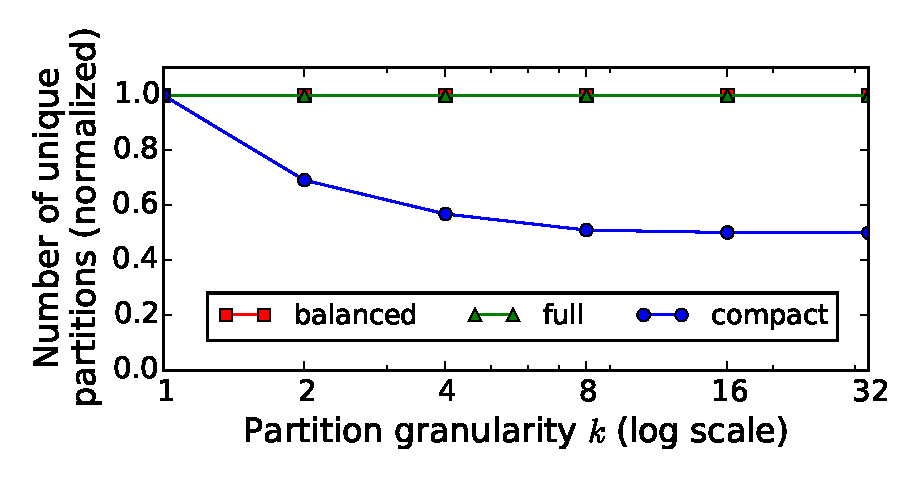
\includegraphics[width=0.8\textwidth]{figures/E42_simulation_colors_resized_powerlaw.eps}
    \caption{The number of unique partitions per node (storage footprint) under different placement schemes.}
    \label{fig:simulation_colors}
\end{figure}

\subsubsection{Storage Footprint}
There are $S=Nk$ choices for placing a partition replica.
When placing multiple replicas of the same partition on the same node,
it reduces the number of unique partitions per node.
When the number of unique partitions per node is lower,
it generally requires lower storage footprint.
A lower storage footprint reduces memory pressure, and may lead to higher cache efficiency.
We run a set of simulations with $M=64$, $R=2$ and various $k$.
This work only presents the results of the \emph{power law} workloads.
Other workload cases show very similar effects.

\myfigure{\ref{fig:simulation_colors}} shows the average number of
unique partitions on each node.
By definition all partitions in 
\emph{full} are unique and it is always 1 (normalized).
\emph{Balanced} is very nearly 1 in all cases.
On the other hand, as $k$ increases, 
\emph{compact} tends to $0.5$, which is $1/R$.
We further investigate how the replication factor affects storage footprint.
\myfigure{\ref{fig:simulation_colors_replication}} shows that the
number of unique partitions tends to $1/R$ as $k$ increases,
which is the desired outcome of the \emph{compact} scheme.


\begin{figure}[!htbp]
    \centering
    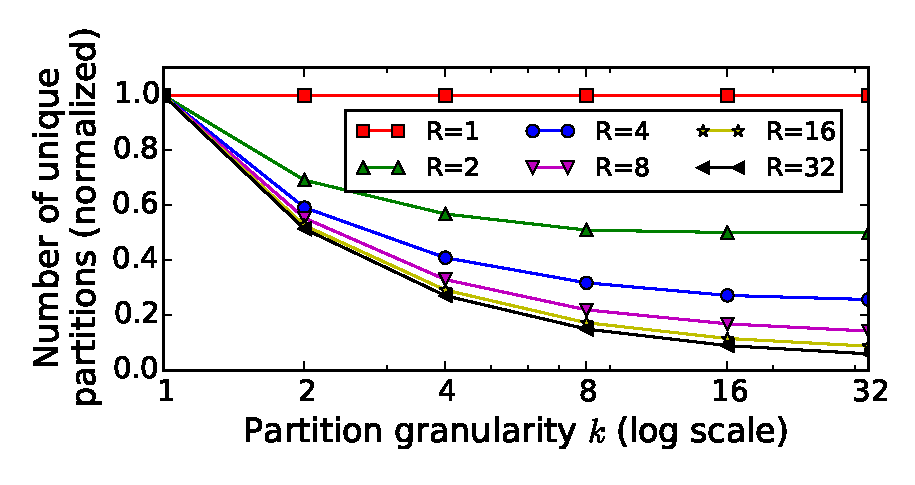
\includegraphics[width=0.8\textwidth]{figures/E42_simulation_colors_replication_resized_powerlaw.eps}
    \caption{The number of unique partitions per node under the \emph{compact} method with various $k$.  The number converges at $k=32$, which is equal to $1/R$.}
    \label{fig:simulation_colors_replication}
\end{figure}

\section{Evaluation}
\label{sec:evaluation}

This section presents our evaluation.
We introduce our experimental setup and benchmark
design.
We then evaluate different placement schemes
by measuring query throughput and
testing their robustness to slight workload mispredictions.


\subsection{Experiment Setup}

We conducted our evaluation on Virtual Computing Lab (VCL), a cloud
platform provided by NC State University.
All servers are equipped with 2-core Intel Xeon CPU and 8GB memory
and connected to a 10 Gbit switch. 
VCL only provides limited storage capacity of local disks or
\emph{instance storage}.
This is also the case for many cloud configurations.
In fact, a majority of EC2 instance types in Amazon Web Services (AWS) do not
have any instance storage.
Instead one must mount a remote volume served by a enterprise-level
storage system.
(AWS calls this \emph{elastic block storage}--EBS.)
We evaluate our approach using both instance storage (local disks) and
remote volumes provided by network file system (NFS),
backed by NetApp 2554 filer with dual controllers.

We evaluate our placement schemes on
high performance computing cluster (HPCC)~\cite{middleton2011hpcc}.
HPCC is an open source
data analytics computer developed by LexisNexis Risk
Solutions for processing big data.
They maintain several clusters with more than 100 nodes, the largest
with more than 500, to provide services to their clients.
Experiments were conducted on a HPCC Roxie cluster.
Roxie is a \emph{data delivery engine} that responds to queries.
It finds the answers to requests in an index that is partitioned and,
if desired, replicated across the nodes.
Roxie is optimized to handle massive amounts of concurrent requests
with low latency.

Data replication and placement that fit workload demands
have direct performance impact on performance.
Roxie clusters partition and distribute data
with two replicas per partition by default.
We modified Roxie to incorporate our data placement schemes.
Our approaches are not specific to Roxie.
They should be able to apply to
Apache Hadoop, HBase, Cassandra, and Ceph, providing benefit when
workloads are not uniformly distributed across
keys, partitions or nodes.


\subsection{Workload Generator and Benchmark Suite}

To evaluate the results learned in our simulation, we developed a
distributed benchmark tool 
that is able to issue a large volume of concurrent queries to
Roxie. 
This benchmark tool adopts the master-slave architecture, where
the the master node generates workload according to a workload profile, and
the slave nodes execute the query requests.
This tool is customizable and supports any number of
workload distributions.
This benchmark suite is written in Python, and designed for testing
query performance at large scale.

In our evaluation, we are interested in how placement schemes
with different levels of partition granularity
respond to different types of workload distribution.
We consider \emph{uniform}, \emph{beta}, \emph{power law}, \emph{normal}, and \emph{gamma} distributions.
The beta distribution is defined on the interval $[0, 1]$ with
two shape parameters, $\alpha$ and $\beta$.
We choose $\alpha=2$ and $\beta=2$ for the base case of beta distribution. 
The power law distribution is controlled by the
\emph{shape} parameter and we choose $3$ for the base case.
Regarding the normal (or Gaussian) distribution it has a
\emph{mean} and a \emph{standard deviation} parameter, which is
$0$ and $1$ in our case.
The gamma distribution also has a \emph{shape} parameter and the base case
uses $5$.
%\ick[redundant?] -> we didn't specify the parameters in detail.
A single instance of each workload is used in all the empirical tests
of Roxie so that results can be compared across multiple runs and
different configurations.
The specific workloads used are those shown in
\mytable{\ref{tab:load-imbalance}}.


\subsection{Benchmark Steps}

To best measure the performance, our benchmark service runs
one worker node for each Roxie server, which 
eliminates the performance impact at the client side.
We use separate machines from the Roxie cluster on the VCL for the benchmark service.
The Roxie controller node dispatches requests and synchronizes with workers.
Worker nodes request jobs and execute them as soon as possible.


We generate the five workload distributions
with different access counts to keys.
All datasets are 128GB.
Next, we specify the smallest cluster size $M$,
the replication factor $R$ (which determines
the cluster size $N$), and
the partition granularity $k$.
In our evaluation, $M$ is equal to 4.
The coarse-grain schemes replicate data on
a node basis.
Fine-grain schemes, on the other hand,
divides the data on a node into 32 equal-size partitions
(1GB per partition).

We compare five placement schemes in total.
First, \emph{base} represents the uniform data placement.
It is coarse grain ($k=1$) and not workload aware.
The \emph{coarse} scheme is also coarse-grain but replicates partitions
based on anticipated workload.
For the fine-grain schemes ($k=32$), we consider
\emph{compact} to reduce storage footprint while maximizing cache locality,
and \emph{balanced} to minimize load imbalance among machines.
In our evaluation, we found that the \emph{balanced} and \emph{full} scheme
have comparable performance.
Due to the page limit, we report the results of \emph{balanced} in most cases.
Last, the \emph{complete} is an ``idealistic'' placement where each
node holds the entire dataset.
It represents an upper bound.

\begin{table}[t]
\centering
\caption{Steady-State Throughput Comparison (instance storage)}
\resizebox{\columnwidth}{!}{%
\begin{tabular}{llllll}
\toprule
{} &  Uniform & Beta &  Power Law & Normal  &   Gamma \\
\midrule
\emph{base}          & 394.8            &  353.5            &  206.6             &    290.4             &  171.2 \\
\emph{coarse}        & -                &  367.8 ($4.0\%$)  &  381.9 ($84.9\%$)  &    364.0 ($25.3\%$)  &  309.7 ($80.9\%$) \\
\emph{compact}       & 375.4 ($-4.9\%$) &  377.5 ($6.8\%$)  &  383.2 ($85.5\%$)  &    374.6 ($29.0\%$)  &  374.2 ($118.6\%$) \\
%Rainbow       & 388.6 ($-1.6\%$) &  398.8 ($12.8\%$) &  438.7 ($51.1\%$)  &    416.8 ($101.8\%$) &  438.5 ($156.2\%$) \\
\emph{balanced}      & 408.1 ($3.4\%$)  &  412.6 ($16.7\%$) &  422.8 ($104.7\%$) &    442.5 ($52.4\%$)  &  455.9 ($166.3\%$) \\
%MCMLB         & 447.0 ($6.8\%$) &  449.0 ($14.8\%$) &  484.0 ($56.1\%$)  &    460.0 ($119.4\%$) &  483.0 ($201.9\%$) \\
\emph{complete}      & 446.8 ($13.2\%$) &  445.4 ($26.0\%$) &  448.3 ($117.0\%$) &    450.1 ($55.0\%$)  &  447.0 ($161.1\%$) \\
\bottomrule
\multicolumn{6}{r}{unit: queries/second} 
\end{tabular}
}
\label{tab:throughput_comparison_local}
\end{table}


Our next step is to change the data layout in Roxie to reflect
the desired data placement decision.
The Roxie cluster is restarted to load the new data layout.
To avoid cache interference, the file system cache is cleared
before every benchmark run.

Last, a workload profile is submitted to the benchmark controller.
The controller node generates the query plan accordingly.
In this way, the same stream of requests is presented for each
benchmark, which allows us to verify results with multiple identical
runs and to compare results from different placements.
We collect query throughput during the entire benchmark process.

\subsection{Steady-State Throughput}
\label{sec:throughput}

We conduct this evaluation to test steady-state throughput.
We generate 30,000 requests for each of the five workload
distributions.
We then calculate the average throughput over the sampling period
(the first and last $10\%$ period are not included.)
This measurement ensures we capture the stable throughput, but not
the warm-up period (low throughput) and
the long-tail period (system is not saturated).


\begin{figure}[!htbp]
\begin{subfigure}[b]{0.6\textwidth}
    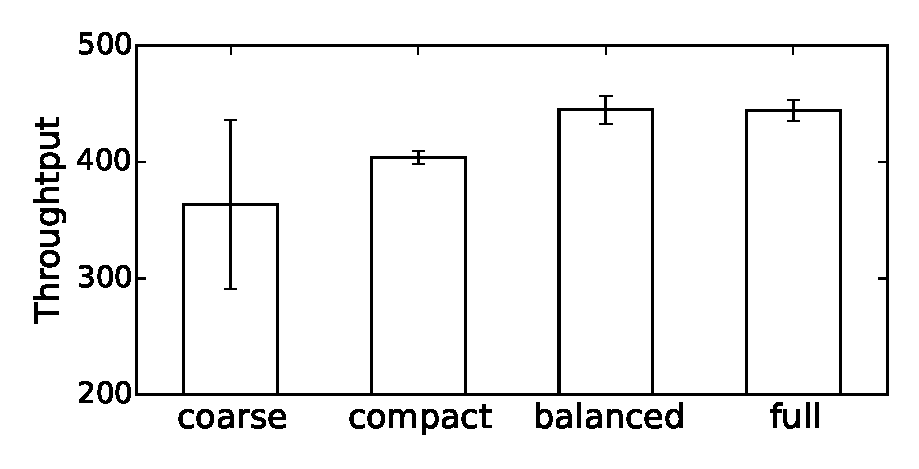
\includegraphics[width=\linewidth]{figures/E38_robustness_std_beta.eps}
    \caption{Beta}
    \label{fig:robustness_beta}
\end{subfigure}
\begin{subfigure}[b]{0.6\textwidth}
    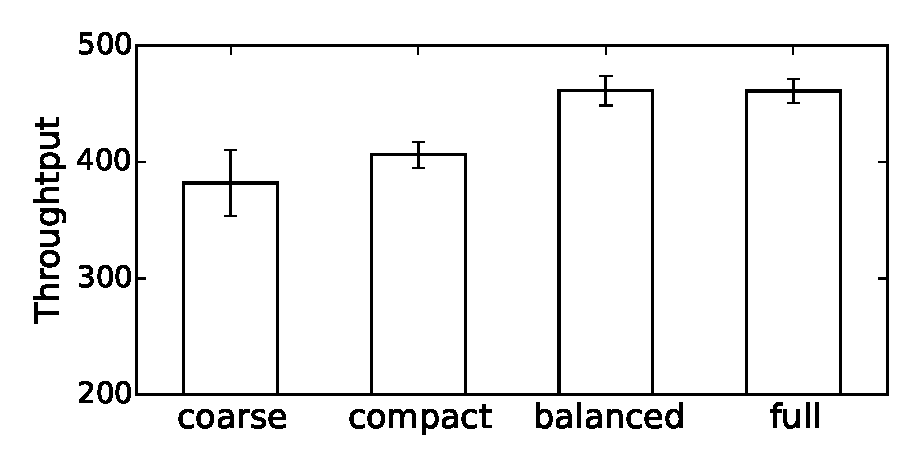
\includegraphics[width=\linewidth]{figures/E38_robustness_std_powerlaw.eps}
    \caption{Power Law}
    \label{fig:robustness_powerlaw}
\end{subfigure}
\begin{subfigure}[b]{0.6\textwidth}
    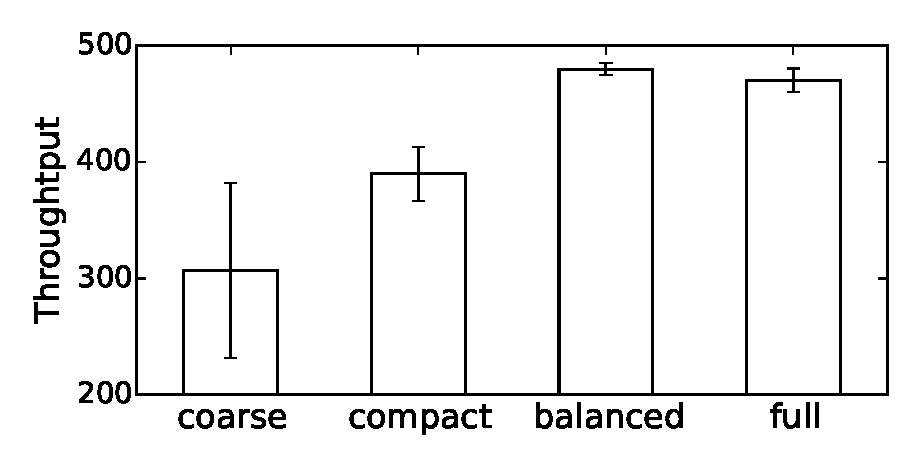
\includegraphics[width=\linewidth]{figures/E38_robustness_std_gamma.eps}
    \caption{Gamma}
    \label{fig:robustness_gamma}
\end{subfigure}
    \centering
    \caption{Compare robustness under slight workload mispredictions. The $y$-axis represents queries per second, and starts from 200 for better presentation to tell performance difference.}
    \label{fig:robustness}
\end{figure}


\subsubsection{Local Storage}

Our evaluation starts with storing data required for Roxie queries
on local disks.
This evaluation involves 8 Roxie nodes: $M=4$ and $R=2$.
\mytable{\ref{tab:throughput_comparison_local}} shows the throughput
of proposed replication and placement schemes under
different workloads.
The values in parenthesis are the speedup relative to \emph{base} performance at
the top of each column.
The \emph{base} placement strategy is uniform.
It does not perform well as
the skewness of workload increases.
For example, the power law workload in the uniform data placement
can only achieve $52.3\%$ of the throughput of a uniform workload.
The second strategy is also coarse grain but replicates according to
anticipated workload.
On a uniform workload this is the same as \emph{base}.
It out performs \emph{base} on skewed workloads.
For example, it
achieves $84.9\%$ more throughput than \emph{base} on \emph{power law}.


Two fine-grain approaches, \emph{compact} and \emph{balanced}, which
further improve performance over \emph{coarse}, are also shown.
In the normal workload case, \emph{compact} and \emph{balanced}
improve on \emph{coarse} by an additional $10.6$ and $78.5$ queries per second.
In the gamma case, \emph{balance} adds $146.2$ queries,
a $47.2\%$ improvement over \emph{coarse}.
Workload-aware data placement is preferable for non-uniform workloads.
The fine-grain strategies out perform \emph{coarse} on all the skewed
workloads.
This is attributed to better load balancing.
As skew increases, the benefit from fine-grain increases (because the
load imbalance in \emph{coarse} increases).


\begin{comment}
\begin{table*}[h]
\centering
\caption{Steady-State Throughput Comparison}
\begin{tabular}{llllll}
\toprule
{} &  Uniform & Beta &  Normal &  Power Law &   Gamma \\
\midrule
Base          & 399.0           &  267.0          &  227.0           &    180.0           &  159.0 \\
Coase         & -               &  368.0 ($38\%$) &  362.0 ($59\%$)  &    371.5 ($106\%$) &  309.5 ($\ \ 95\%$) \\
Monochromatic & 402.5 ($0.9\%$) &  409.0 ($53\%$) &  410.0 ($81\%$)  &    403.5 ($124\%$) &  399.0 ($151\%$) \\
Rainbow       & 426.0 ($6.8\%$) &  431.0 ($61\%$) &  405.5 ($79\%$)  &    442.0 ($146\%$) &  427.0 ($169\%$) \\
Complete      & 438.0 ($9.8\%$) &  414.0 ($55\%$) &  433.0 ($91\%$)  &    449.0 ($149\%$) &  431.0 ($171\%$) \\
\bottomrule
\multicolumn{6}{r}{unit: queries/second} 
\end{tabular}
\label{tab:throughput_comparison}
\end{table*}
\end{comment}


\begin{table}[t]
\centering
\caption{Steady-State Throughput Comparison (NFS)}
\resizebox{\columnwidth}{!}{%
\begin{tabular}{llllll}
\toprule
{} &  Uniform & Beta &  Power Law &  Normal &   Gamma \\
\midrule
\emph{base}       & 446.1            &  383.1            &  220.2             &    393.3             &  176.4 \\
\emph{coarse}     & -                &  396.4 ($3.5\%$)  &  415.3 ($88.6\%$)  &    379.6 ($29.4\%$)  &  327.9 ($85.9\%$) \\
\emph{compact}    & 403.7 ($-9.5\%$) &  416.2 ($8.7\%$)  &  401.3 ($82.3\%$)  &    407.1 ($38.8\%$)  &  407.8 ($131.1\%$) \\
%Rainbow   & 447.3 ($0.3\%$)  &  428.1 ($11.8\%$) &  474.0 ($61.6\%$)  &    469.0 ($113.0\%$) &  481.5 ($172.9\%$) \\
\emph{balanced}   & 447.6 ($0.3\%$)  &  440.8 ($15.1\%$) &  454.0 ($106.2\%$) &    469.7 ($60.1\%$)  &  485.9 ($175.5\%$) \\
%MCMLB     & 447.9 ($0.4\%$)  &  448.8 ($17.2\%$) &  479.8 ($63.6\%$)  &    455.5 ($106.9\%$) &  482.0 ($173.2\%$) \\
\emph{complete}   & 484.2 ($9.0\%$)  &  485.6 ($26.8\%$) &  492.4 ($123.7\%$) &    495.0 ($68.8\%$)  &  490.0 ($177.8\%$) \\
\bottomrule
\multicolumn{6}{r}{unit: queries/second} 
\end{tabular}
}
\label{tab:throughput_comparison_nfs}
\end{table}


The \emph{complete} solution out performs all others, including both fine-grain
solutions.
This is because while the workload was probabilistically generated
over 30,000 requests.
The workload for each small window of requests does not always reflect
the overall workload.
In such cases, \emph{complete} performs better.
However, \emph{complete} is generally not feasible
when dataset is too large to fit into one node.

Overall, workload-aware data placement significantly increases query throughput.
Using fine partition granularity better balances the load.
\emph{Balanced} performs better than \emph{compact}, indicating that
the benefit of a smaller footprint is less than the cost of poorer load
balancing.
The \emph{balanced} scheme is occasionally competitive with \emph{complete}.

\subsubsection{Remote Storage}
Next, we evaluate our proposed schemes against data storing on remote storage.
The Roxie cluster size and the number of benchmark clients remain the same
with the local storage case.
\mytable{\ref{tab:throughput_comparison_nfs}} details the throughput numbers.
This evaluation confirms the general observations seen in the instance
storage test.
However, the throughput is higher using remote storage.
While somewhat counter intuitive, it is not unheard.
This occurs because local storage uses plain commodity disks and the
% not sure the original sentence is grammerly correct
filer uses high-performance disks as well as aggressive caching.
Moreover, the I/O demand does not exceed the capacity of the NFS server.
Therefore, the additional network traffic is not creating a
performance bottleneck.


\subsection{Robustness Comparison}
\label{sec:robustness}

We are interested in how sensitive a placement scheme is to minor
deviations in the anticipated workload.
(Tables~\ref{tab:throughput_comparison_local} and
\ref{tab:throughput_comparison_nfs} show performance degradation for
major deviations.)
We say a placement scheme is more \emph{robust} when the scheme works
well even when the actual workload is slightly different from the
anticipated workload.
We pick different parameters for generating slight workload variance.
For example, we change the shape parameter in the power law distribution.
Therefore, it becomes either less or more skewed.
We create two less and two more skewed workloads for each type.

\myfigure{\ref{fig:robustness}} shows how different placement schemes react
to workload shifts.
The figure shows the average throughput and the standard deviation
 of the placement schemes under the four ``shifted'' workloads
The figure indicates that the coarse-grain scheme
under performs in both average (lower) and deviation (greater)
compared to the fine-grain schemes.

The \emph{compact} scheme is better than \emph{coarse} but its performance is not as
good as the \emph{balanced} scheme.
The \emph{balanced} scheme overall exhibits higher throughput than
\emph{coarse} and \emph{compact}.
More importantly, \emph{balanced} shows consistent standard deviation
in three workloads.
The highest performance degradations in each workload are
$2\%$, $6\%$ and $3\%$
while the \emph{compact} scheme shows
$3\%$, $5\%$ and $14\%$ (increasing as skewness increases) degradation respectively.
% The \emph{balanced} shows $6\%$ performance loss at most.
% balanced
%  - beta: 436.41 vs 444.75
%  - power law: 442.22 vs. 471.82
%  - gamma: 472.98 vs. 487.88
% compact
%  - beta: 396.85 vs. 410.53
%  - power: 388.71 vs. 408.26
%  - gamma: 350.19 vs. 408.02
The above suggests than \emph{balanced} is more robust then
\emph{compact}, which is robust than \emph{coarse}.
There is little difference between \emph{balanced} and \emph{full} in either
average throughput or standard deviation.
This is because there is little difference in the placement of
partitions---that is, the balanced scheme tends to have a high degree of
unique partitions on each node.



\subsection{Micro Benchmark}

We have presented the steady-state throughput in Section~\ref{sec:throughput}.
In this section, we further examine why different placement schemes
lead to large performance difference.

We investigate resource utilization of different placement schemes
for understanding the tradeoff between the \emph{compact} and
\emph{balanced} scheme. 
We collect system statistics
(\textit{dstat}~\cite{dstat} and \textit{cachestat}~\cite{cachestat})
during the entire benchmark runs.
\mytable{\ref{tab:micro_nfs}} presents the system statistics, and
metrics are normalized to the smallest value in each metric group,
except the \emph{max:mean} ratio. 
This normalization better shows the difference between placement schemes.
Except \emph{mean \%CPU}, a system is more efficient when
the metrics listed are small.
These metrics are collected from the benchmark runs under the gamma workload.
Other workloads present very similar trends.

First, we examine CPU utilization across all Roxie nodes.
The average CPU utilization indicates whether Roxie is fully saturated,
and the \emph{max:mean} metric tells whether loads are well balanced
among Roxie nodes.
In the \emph{base} scheme, CPU utilization is the lowest and load imbalance
is the highest, which explains why uniform data placement under performs.
Workload-aware replication eliminates load imbalance while
improving CPU utilization.
Fine-grain partition further reduces load imbalance,
as in the \emph{balanced} scheme.

\begin{table}[ht]
\centering
\caption{Normalized System Statistics of Roxie Servers}
\resizebox{\columnwidth}{!}{%
\begin{tabular}{lllllll}
\toprule
	& Metrics	&	\emph{base}	&	\emph{coarse} & \emph{compact} & \emph{balanced} & \emph{complete} \\
\midrule
\multirow{2}{*}{Load Balancing} & \% CPU (mean)		& \textbf{1.00} (13\%) & 2.29   & 2.37 & 3.11 & 2.97     \\
		                        & \% CPU (max:mean) & 2.01 & 1.34   & 1.23 & 1.1    & 1.14     \\
\midrule
\multirow{3}{*}{Cache Locality} & cache misses (sum)     & 1.13 & 1.24   & \textbf{1.00} (659K) & 1.26 & 1.22     \\
		                        & dirty pages (sum)     & 1.20 & 1.47   & \textbf{1.00} (200K) & 1.52 & 1.29     \\
		                        & cache sizes (max) & 2.11 & 1.51   & \textbf{1.00} (825MB)   & 1.17 & 1.15     \\
\midrule
\multirow{2}{*}{Efficiency}     & I/O wait (mean) & 1.39 & 6.73   & \textbf{1.00} (2.35\%) & 2.48 & 2.55     \\
		                        & TCP connections (mean)   & 2.40 & 1.53   & 1.31 & 1.10 & \textbf{1.00} (1357) \\
%		                        & disk read         & 2.72 & 2.00   & 1.09 & \textbf{1.00} & 3.48    \\
\bottomrule
\end{tabular}
}
\label{tab:micro_nfs}
\end{table}



Second, we examine the benefits of packing multiple replicas into the same node,
as in the \emph{compact} scheme.
\mytable{\ref{tab:micro_nfs}} shows that cache misses and dirty pages
are significantly lower in the \emph{compact} scheme.
Besides, \emph{compact} has much lower cache sizes, $17\%$ lower than
\emph{balanced} and $51\%$ less than the \emph{coarse} scheme.
Although the \emph{compact} scheme outperforms others in cache locality and
requires less cache,
it does not generate the highest query throughput.
A possible explanation is that requests do not greatly benefit from better cache locality.
We suspect the \emph{compact} scheme is useful especially when query applications
require costly read operations.
% We will need to further investigate this case.

Third, we compare I/O wait time and the number of TCP connections
for comparing their efficiency.
A lower I/O wait time indicates that systems do not waste much time on slow I/O operations.
The \emph{compact} scheme, with maximum cache locality, has the lowest I/O wait value.
The number of TCP connections at a given time is related to processing efficiency.
We observe that the \emph{balanced} scheme yields a lower number of TCP connections
than the other schemes, suggesting that requests complete more quickly.


\subsection{Summary}
Our evaluation provides empirical data to support our findings
in the simulation.
First, workload-aware data placement, both the coarse and fine grain methods,
reduces load imbalance, thereby improving system throughput.
However, the coarse-grain approach is insufficient
when workload is highly skewed.
Finer partitioning further balances the loads and in many cases,
the \emph{balanced} scheme has comparable performance to \emph{complete}
(an ``idealistic'' placement).
Furthermore, both \emph{balanced} and \emph{full} are robust while
\emph{compact} reduces storage footprint to $1/R$. 



%% 
\section{Related Work}
\label{sec:related}

The data replication and placement issues have been extensively studied
in several research domains
including memory cache~\cite{Leff1993,Zaman2011},
distibuted storage systems~\cite{Lim2010},
NoSQL database~\cite{Rodrigues2013,Cruz2013,Corbett2013}
traditional retaional databases~\cite{Pavlo2012,Curino2010},
content delivery network (CDN)~\cite{Laoutaris2006}, etc.

Data replication is a common technique to increase
system performance and availability.
Many distributed systems use multiple replicas to
increase reliability and availability as well as improve system
performance~\cite{hbase,SageWeil2006Ceph}.
This chapter focuses on data replication and
its impact on system performance.
Data placement, on the other hand, determines the locations of data.
Apache Hadoop, for example, writes a replica locally and
two replicas in another rack to improve
system performance~\cite{Xie2010,Eltabakh2011}.
Our work makes contributions in three ways.
First, partition granularity determines the basic unit to calculate load.
Second, data replication is governed by anticipated workload.
Last, data placement chooses the slots on servers for maximizing
load balancing or exploiting cache locality.

Ceph is a distributed storage system
that supports configurable replication factors
for the placement group~\cite{SageWeil2006Ceph}.
Similarily, Apache Hadoop~\cite{hadoop} accepts separate replication factors
for different data chunks.
Optimizing the number of replications per object or data chunk
is a challenging task.
AptStore proposes the Popularity Prediction Algorithm (PPA) by
analyzing file system logs and adjusts replication factors accordingly
for files on Apache Hadoop~\cite{Krish2013}.
Scarlett combines offline log analysis and online prediction to
accurately estimate block popularity~\cite{Ananthanarayanan2011}.
Results show that replicating hotter data avoids bottlenecks,
thereby improving the performance of MapReduce jobs.
% These works greatly improve distributed storage performance but
% do not totally answer all the essential properties of
% data replication and placement.

The NoSQL database is a popular repository for large-scale data
because of they support extreme horizontal
scaling~\cite{Lakshman2010,Chang2008,hbase,mongodb}.
%\cmt{add more citations, eg, hbase, reddis,dynamodb, mongodb.}
Studies have shown that non-uniform query key
causes performance issues.
AUTOPLACER \cite{Rodrigues2013} optimizes the placement
for the top-k objects in the distributed key-value store.
To minimize the maintenance cost of large number of objects,
AUTOPLACER proposes the probabilistic data structure (PAA)
to reduce routing latency.
MET \cite{Cruz2013} is an elasticity framework that 
optimizes data placement to fit workload characteristics for HBase.
It is able to reconfigure HBase dynamically when an HBase cluster
requires expansion or contraction.
MET found that heterogeneous machines can easily lead to load imbalance.
To balance the load on each server, MET groups data partitions
according to their access pattern.
MET models the cost of placing data partitions on nodes, and
uses Longest Processing Time (LPT) to minimize the cost,
which maximizing load sharing among nodes.
%\cmt{what is makespan?}
The above implements a system that replicates and places data according to
data access pattern.
Our work explores how data replication and placement schemes
affect system performance under different workload distribution.

%%%%%%%%%%%%%%%%%%%%%%%%%%%%%%%%%%%%%%%%%%%%%%%%%%%%%%%
% moved fig this from model.tex to make it float to first page of mode
%%%%%%%%%%%%%%%%%%%%%%

%%%%%%%%%%%%%%%%%%%%%%%%%%%%%%%%%%%%%%%%%%%%%%%%%%%%%%%

Elastic storage dynamically expands or contracts a storage cluster.
The elastic controller is responsible for
provisioning resources and adjusting data replication and placement
for efficient storage configurations.
The SCADS director \cite{Trushkowsky2011} is an elastic controller
that automatically scales out a storage system to meet stringent
performance requirements. 
SCADS adopts a model-based approach to correlate request workload and
latency. 
It keeps track of the hottest bins (groups of data), and
dynamically moves these bins to different servers for balancing the load.
SCADS also creates performance models to predict workload and server capacity
for better estimating query latency.
Lim et al. propose a design of elastic storage\cite{Lim2010}.
Scaling a storage system poses challenges such as actuator delays,
measurement accuracy and interference with applications.
Their work puts emphasis on the elastic controller, whereas
we discover the relationship between
workload characteristics and data placement
when scaling a data-intensive application.

Sharding is a common technique to distribute load by
partitioning data across distributed server nodes.
More specifically, sharding is an approach that partitions data
according to keys, where partitions are placed
on different servers independently~\cite{Cattell2011}.
This horizontal scaling enables a distributed system to scale efficiently.
NoSQL databases, such as BigTable~\cite{Chang2008}, HBase~\cite{hbase}
and Cassandra~\cite{Lakshman2010}, rely on sharding
to efficiently balance load.

For relational databases, sharding is heavily used to support
a large volume of queries.
Schism uses graph-partitioning algorithms
to determine the optimal partitioning
for minimizing the cost of distributed transactions~\cite{Curino2010}.
The proposed fine-grained data partition minimizes
the required number of distributed transactions for database applications.
Pavlo \emph{et al}. develop a database tool that is able to generate
optimal database designs for parallel OLTP systems~\cite{Pavlo2012}.
They propose a new search algorithm for partitioning database and
create a cost model to minimize the coordination cost
while maximizing load balance.
Spanner is a semirelational database that
manages replicated data globally and performs resharding
at runtime for better load balancing~\cite{Corbett2013}.
Slicer is an auto-sharding service designed by Google~\cite{Adya2016}.
To leverage Slicer, users are required to
associate incoming requests with a key.
Slicer dynamically maps the key to a proper task
for maximizing load balance.
The above studies implement either
a sharding mechanism or design s generic sharding service,
while our work focuses on understanding the tradeoff
between different data placement schemes
when data partitions required proper placement to
meet workload distribution.

\section{Conclusion}
\label{sec:conclusion}

Efficient deployment of large-scale, distributed systems with
an irregular workload requires both cluster sizing and data placement.
We show the uniform distribution is (unsurprisingly) poor for
typical, non-uniform workloads.
This work further shows that coarse-grain replication can reduce
over-utilization but is unable to address under-utilization.
Finer partition granularity reduces both under- and
over-utilization.
With fine-grain partitioning there is a placement decision.
Maximizing the number of unique partitions per node increases robustness
to workload misprediction,
while minimizing the number reduces storage
footprint.
Our empirical study using an HPCC Roxie cluster shows
the benefit of footprint reduction does not offset cost due to poorer
load balancing.
However, we do not believe this is universally true.

This work focuses on the dimension and tradeoffs of various data
replication and placement strategies.
For our future work, we plan to implement an elastic controller
that incorporates our proposed data placement schemes.
In an elastic system, the gains of the optimal placement must be
offset by the cost of data movement.
Calculating this data movement cost remains as a future work.
